\documentclass[12pt]{article}
\usepackage{amsmath,amsthm,amssymb,amsfonts,setspace,tikz}

\textwidth 7.0 truein
\oddsidemargin -0.25in   %left-hand edge
\evensidemargin -0.5 truein  %right-hand edge
\topmargin -0.85in      %top of paper to top of head, pulls whole unit
\textheight 9.5in

%%%% In most cases you won't need to edit anything above this line %%%%

\begin{document}
\hfill Name 

\hfill Math 2270

\hfill Assignment \#

\section*{Problem Set 1.1}

\begin{itemize}

\item[\textbf{1}] Describe geometrically

Solution

(a)
$
u\begin{bmatrix} 1 \\ 2 \\ 3 \end{bmatrix}
+
v\begin{bmatrix} 3 \\ 6 \\ 9 \end{bmatrix}
=
\begin{bmatrix} (u+3v) \\ 2(u+3v) \\ 3(u+3v) 
\end{bmatrix}
$

\item[\textbf{2}] Draw in single plane

Solution

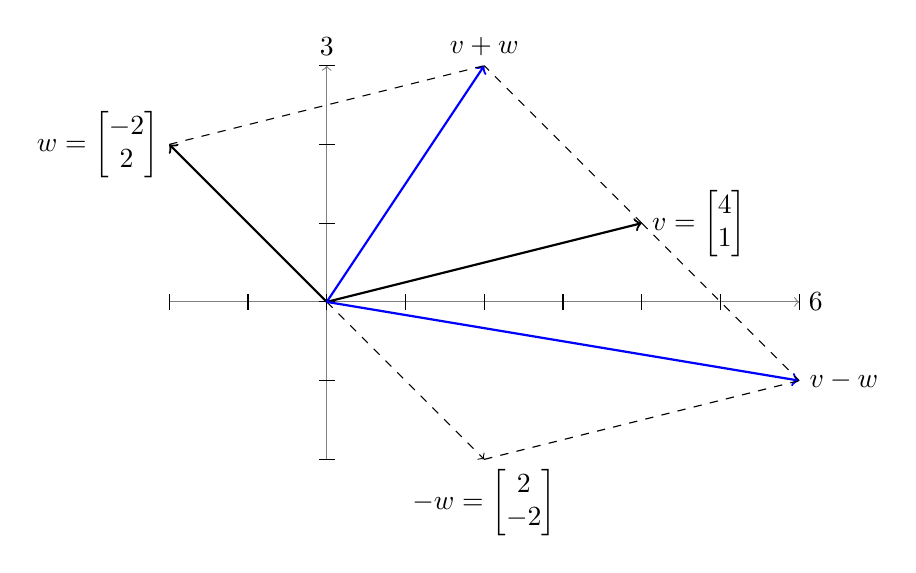
\begin{tikzpicture}
	\coordinate (o) at (0,0);
	\coordinate (v) at (4,1);
	\coordinate (w) at (-2,2);
	\coordinate (-w) at (2,-2);
	\coordinate (sum) at (2,3);
	\coordinate (diff) at (6,-1);

	\draw [thin, gray, ->] (0,-2) -- (0,3)
		node [above, black] {$3$};

	\draw [thin, gray, ->] (-2,0) -- (6,0)
		node [right, black] {$6$};

	\foreach \x in {-2,...,6}
		\draw (\x,0.1) -- (\x,-0.1);
	\foreach \y in {-2,...,3}
		\draw (0.1,\y) -- (-0.1,\y);

	% \filldraw [gray] (v) circle (2pt);
	\draw [thick, black, ->] (o) -- (v)
		node [right, black] {$v=\begin{bmatrix} 4 \\ 1\end{bmatrix}$};

	% \filldraw [gray] (w) circle (2pt);
	\draw [thick, black, ->] (o) -- (w)
		node [left, black] {$w=\begin{bmatrix} -2 \\ 2\end{bmatrix}$};

	\draw [thick, blue, ->] (o) -- (sum)
		node [above, black] {$v+w$};
	\draw [dashed] (v) -- (sum);
	\draw [dashed] (w) -- (sum);

	\draw [dashed, ->] (o) -- (-w)
		node [below, black] {$-w=\begin{bmatrix} 2 \\ -2\end{bmatrix}$};

	\draw [thick, blue, ->] (o) -- (diff)
		node [right, black] {$v-w$};
	\draw [dashed] (v) -- (diff);
	\draw [dashed] (-w) -- (diff);
\end{tikzpicture}

\item[\textbf{3}] Compute and Draw

Solution

$
v + w = \begin{bmatrix} 5 \\ 1 \end{bmatrix}, v - w = \begin{bmatrix} 1 \\ 5 \end{bmatrix}
v = \begin{bmatrix} 3 \\ 3\end{bmatrix}, w = \begin{bmatrix} 2 \\ -2\end{bmatrix}
$

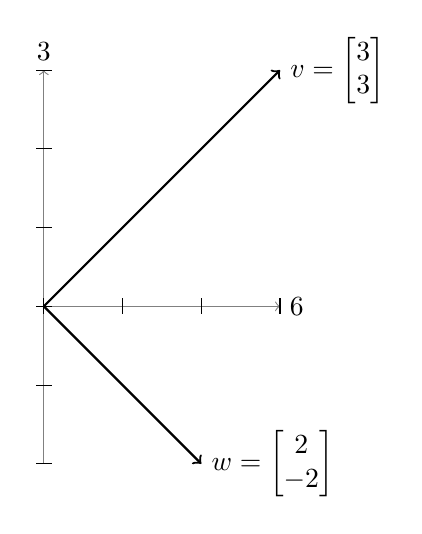
\begin{tikzpicture}
	\coordinate (o) at (0,0);
	\coordinate (v) at (3,3);
	\coordinate (w) at (2,-2);

	\draw [thin, gray, ->] (0,-2) -- (0,3)
		node [above, black] {$3$};

	\draw [thin, gray, ->] (0,0) -- (3,0)
		node [right, black] {$6$};

	\foreach \x in {0,...,3}
		\draw (\x,0.1) -- (\x,-0.1);
	\foreach \y in {-2,...,3}
		\draw (0.1,\y) -- (-0.1,\y);

	\draw [thick, black, ->] (o) -- (v)
		node [right, black] {$v=\begin{bmatrix} 3 \\ 3\end{bmatrix}$};

	\draw [thick, black, ->] (o) -- (w)
		node [right, black] {$w=\begin{bmatrix} 2 \\ -2\end{bmatrix}$};
\end{tikzpicture}

\item[\textbf{4}] Find components

Solution

$
v = \begin{bmatrix} 2 \\ 1 \end{bmatrix}, 
w = \begin{bmatrix} 1 \\ 2 \end{bmatrix}
$

$
3v+w = \begin{bmatrix} 3*2+1 \\ 3*1+2 \end{bmatrix} = \begin{bmatrix} 7 \\ 5 \end{bmatrix}, 
cv+dw = \begin{bmatrix} c*2+d*1 \\ c*1+d*2 \end{bmatrix} = \begin{bmatrix} 2c+d \\ c+2d \end{bmatrix}
$

\item[\textbf{5}] Find components

Solution

$
u = \begin{bmatrix} 1 \\ 2 \\ 3 \end{bmatrix}, 
v = \begin{bmatrix} -3 \\ 1 \\ -2 \end{bmatrix},
w = \begin{bmatrix} 2 \\ -3 \\ -1 \end{bmatrix}
$

$
u + v + w = \begin{bmatrix} 0 \\ 0 \\ 0 \\ \end{bmatrix}
$

$
2u + 2v + w = \begin{bmatrix} -2 \\ -2 \\ 0 \\ \end{bmatrix}
$

$
w = -u + -v \implies w \text{ is on the same plane as } u \text{ and } v
$

\item[\textbf{6}] Find $c$ and $d$

Solution

$
v = (1,-2,1), w = (0,1,-1) \\
\implies cv + dw = (c, -2c + d, c - d) = (3,3,6) \\
\implies \begin{matrix} c = 3 \\ d = 9 \\ c - d = 6 \end{matrix}
\implies \text{no solution because $6 \neq 6$}
$

\item[\textbf{7}]

\item[\textbf{8}] Sum of two diagonals

Solution

$
\text{sum diagonal } v + w = (3,4) \\
\text{difference diagonal } v - w = (5,0) \\
\text{sum of 2 diagonals } 2v = (8,4)
$


\item[\textbf{9}] Possible 4th corners

Solution

$
(1,1)\text{, }(4,2)\text{ and }(1,3)
$

$
u-o=(v-o)+(w-o)
\implies u=v+w-o
\implies 3\text{ possible o }
\implies 3\text{ 4th corners}
$

\item[\textbf{10}] describe $(x,y,z)$ in cubes

Solution

$
i=(1,0,0)\text{, }j=(0,1,0)\text{ and }k=(0,0,1)
$

$
$

\item[\textbf{11}] 
\item[\textbf{12}]
\item[\textbf{13}]
\item[\textbf{14}]
\item[\textbf{15}]



\item[\textbf{16}]
\item[\textbf{17}]
\item[\textbf{18}]
\item[\textbf{19}]
\item[\textbf{20}]
\item[\textbf{21}]
\item[\textbf{22}]
\item[\textbf{23}]
\item[\textbf{24}]
\item[\textbf{25}]
\item[\textbf{26}]
\item[\textbf{27}]
\item[\textbf{28}]
\item[\textbf{29}]
\item[\textbf{30}]
\item[\textbf{31}]

\end{itemize}

\end{document}
